
%
%\section{Core Layout}
%There are 24 cores on the available machines. 12 cores are available on each NUMA socket.
%Although there are 2 CPUs (2 hardware threads) available on each core, hyperthreading is
%kept off for reducing the non deterministic behavior attributed to contention of hardware units
%and getting repeatable results.
%
%NUMA- node 1 with starting core 12 is currently used by the RAN.
% \begin{figure}[htbp]
%    \centering
%    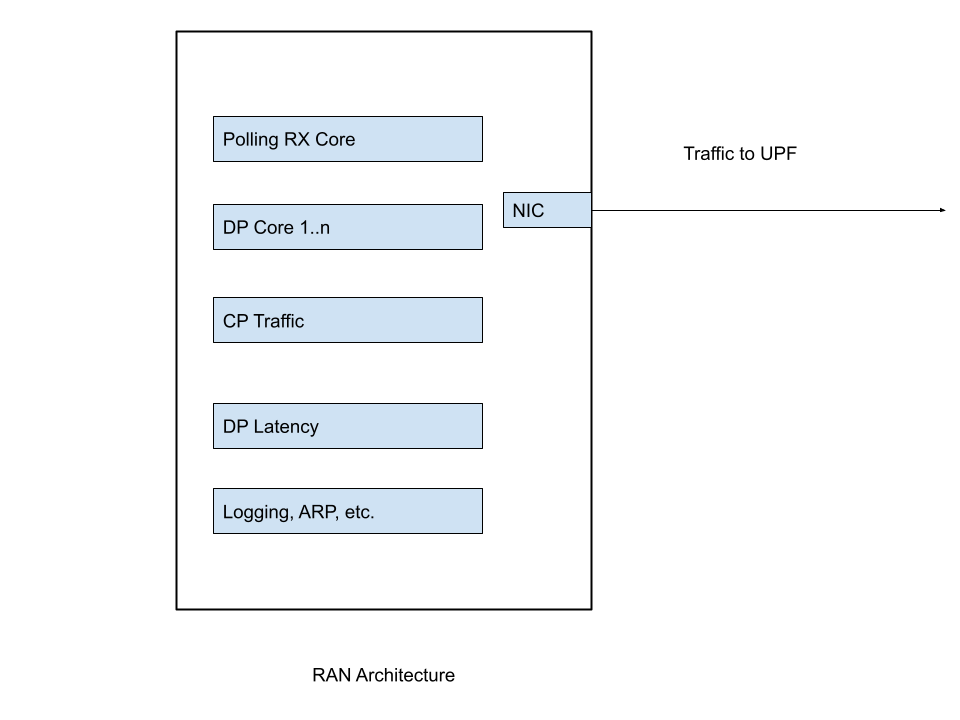
\includegraphics[width=0.8\textwidth, keepaspectratio]{./fig/Introduction/RANArchitecture.png}
%    \caption{RAN Architecture}
%    \label{fig:RAN}
%\end{figure}
%
%\begin{itemize}
%	\item \textbf{CORE\_RX\_POLL}: Receives all the incoming packets from UPF. These includes the latency packets or data packets in the downlink direction.
%	\item \textbf{CORE\_TX\_START - CORE\_TX\_END}
%	      These cores are used to send data packets in the uplink  direction i.e. from RAN to UPF.
%	\item \textbf{CORE\_RTT}
%	      This core sends the data plane latency packets in the uplink direction. These packets are reflected back by the DNN so that end to end latency can be measured.
%	\item \textbf{CORE\_CP\_TRAFFIC} This core sends the control plane traffic. A separate core was used so that a call back can be registered for storing timestamps. These timestamps are used for calculating control plane latency.
%	\item \textbf{CORE\_MISC and CORE\_STAT}
%	      These cores handles miscellaneous functions like ARP handling, timer and logging of stats.
%\end{itemize}
%Using this layout, a maximum of 7 cores are available for the data forwarding on the same numa node.
%To increase this number, the functions running on CORE\_MISC and CORE\_STAT can be run parallely on the same core. Although 7 cores have been found sufficient till now to saturate 40 Gig line with 64 byte packets.
%
%\section{Forwarding of Control Plane Messages}
%In a 5G-conforming RAN, the session related messages are sent by SMF to UPF.
%This RAN-emulator's primary role is that of a load generator. Session related messages - session establishment, modification and release messages are directly sent by RAN to the UPF.
%
%The reasons for making this approximation of behavior is 
%\begin{itemize}
%	\item All the network functions besides UPF and DNN run on the same physical machine in our setup (define this in results). So the approximation is not way off the mark. 
%	\item It is possible to increase the load substantially using DPDK APIs that are used by RAN.
%\end{itemize}
%
%
%
%\section{Modes of Operation}
%The load generator can be used in different modes to characterize the different behaviors of the user plane function. The various modes are
%\begin{itemize}
%	\item Setup Sessions and Send Data.
%	\item Send only control plane traffic.
%	\item Send Control Plane and Data Plane traffic simultaneously.
%	\item Helper functions.
%	\item QoS functions.
%\end{itemize}
%\subsection{Setup sessions and send data}
%Initially sessions are setup by sending session establishment and session modification messages directly from the RAN to the UPF.
%Once the sessions are setup the data packets are forwarded from CORE\_TX\_START- CORE\_TX\_END (inclusive).
%Control plane latency is calculated during the initial setup for all the session related packets. Throughput is also logged in the log file.
%The number of UEs/sessions that are used for sending data per core is asked to the user. The sessions are partitioned in disjoint sets among the cores before forwarding.
%
%\subsection{Send only control plane traffic}
%This mode is used to send only control plane traffic and no data plane forwarding takes place.
%This is a synthetic traffic i.e. it does not represent any real world scenario. The main motive behind this mode was to saturate control plane and measure control plane handling capabilities of the different designs of the UPF. The latency and throughput values are logged in the file as earlier.
%This is an open load test in which session establishment, release and modification 
%packets are sent one by one with a user provided inter packet delay (in us). These 
%packets are sent from CORE\_CP\_TRAFFIC. The open load means that the RAN does not 
%wait for response packets before sending the next packet.  Ideally modification 
%message should be sent only once the session establishment response is received. 
%However, open load is a good approximation of the actual behavior and is easy to
% implement.
%
%\subsection{Send Control Plane and Data Plane Traffic Simultaneously}
%This feature is discussed in Chapter \ref{chap:CPDPTraffic}
%
%\subsection{Helper Functions}
%There is only one helper function right now. This helper function - Delay Estimator - helps in mapping inter batch delay with the data forwarding throughput of the load generator for a given number of cores and sessions.
%This mapping is used to set the rate of forwarding of the data packets. Intel 40Gbps NICs that we have do not have rate limiting APIs like 10Gbps NIC.
%
%\subsection{QoS Functions}
%These functions were developed to check the correctness of QoS algorithms deployed at the UPFs. These functions were tested on 10Gbps NIC systems and may require modification for other NICs.
%
%
%For QoS testing, it was required to test whether the packet forwarding rate is actually limited by
%the algorithm. For this, data is forwarded at a low rate and at a high rate. The low rate is lower than  the rate limit imposed on the sessions. The high rate is higher than the limit. So when the rate is higher, the output at UPF is limited to the rate limit.
%
%Lower rate - 700 Mbps, High rate - 1200 Mbps, Rate limit -1000 Mbps. When the incoming rate at the UPF is 1200 Mbps, outgoing rate is 1000 Mbps if the QoS algorithm is correct.
%
%